\documentclass[11pt,a4paper,roman]{scrartcl}
\usepackage{parskip}
\usepackage[english]{babel}
\usepackage{url}
\usepackage[utf8x]{inputenc}
\usepackage{amsmath}
\usepackage{amssymb}
\usepackage{graphicx}
\usepackage[export]{adjustbox}
\usepackage{listings}
\usepackage{float}
\usepackage{hyperref}
\usepackage[document]{ragged2e}
\usepackage{bm}
\usepackage[section]{placeins}
\title{Computer exercise 2}
\date{}
\author{Carl Ridnert, 940325-0112, ridnert@kth.se \\
Yue Jiao, 911024-7799, yj@kth.se}


\begin{document}
\maketitle
\begin{figure}[h]
\centering

\includegraphics[width=0.45\textwidth,center]{KTH_CMYK}
\end{figure}
\newpage


\section*{2.1.1}

In this problem, the followng RK3 method is given:

\begin{equation}
\begin{aligned}
\centering
u_k & =u_{k-1}+\frac{h}{6}(K_1+K_2+4K_3),\quad t_k=t_{k-1}+h, \quad k=1,2, ..., N \\
K_1 & =f(t_{k-1},u_{k-1})\\
K_2 & =f(t{k-1}+h,u_{k-1}+hK_1)\\
K_3 & =f(t_{k-1}+h/2,u_{k-1}+hK_1/4+hK_2/4) 
\end{aligned}
\end{equation}


This is implemented on Van der Pol's differential equation

\begin{equation}
\frac{d^2y}{dt^2}+(y^2-1)\frac{dy}{dt}+y=0, \quad y(0)=1, \quad \frac{dy}{dt}(0)=0, \quad \epsilon=1, \quad t\in [0,1].
\end{equation}

By setting $u_1=y$ and $u_2=\frac{dy}{dt}$ one sees that the differential equation can be written as a system of first order ODE's as follows.

\begin{equation}
f(u) =\begin{bmatrix}
  \frac{du_1}{dt} \\
  \frac{du_2}{dt}
 \end{bmatrix}=
 \begin{bmatrix}
 0 & 1 \\
 -1 & 1-u_1^2
 \end{bmatrix}
 \begin{bmatrix}
 u_1 \\
 u_2
 \end{bmatrix}
\end{equation}

The recursion for $u_k$ in (1) is computed in the time interval $[0,1]$ and made for a varying number of steps $N=1/h$, taking the following values: $N=[10\quad20\quad 40\quad 80\quad 160\quad 320]$.\\

The error at $t=1,e_N=y_N-y(1)$ is then estimated by $\hat{e}=u_N-u_{320}$. This error can be plotted in a loglog-plot as a function of the step size h, which is shown in figure 1.

\begin{figure}[h]
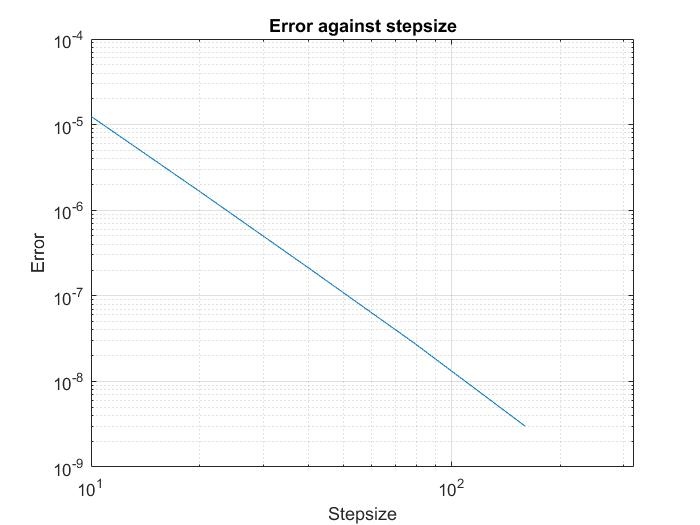
\includegraphics[width=0.7\textwidth,center]{1}
\caption{Loglog plot of $|e_N|$ as a function of the step size h.}
\end{figure}

From this, it is apparent that the error decreases as the step size decreases. The order is the k-value of the slope in the loglog plot which can be estimated directly from the graph.

One rough estimate is:

\begin{equation}
k=\frac{log(\frac{0.5*10^-5}{0.4*10^-8})}{log(\frac{0.1}{0.01})}\approx3
\end{equation}

From which one can conclude that the method is of order 3.

\newpage
\section*{2.1.2}
In this problem the following equation system shall be solved with different methods. 

\begin{equation}
\begin{aligned}
\frac{dx_1}{dt} &= -k_1 x_1 + k_2 x_2 x_3, \qquad x_1(0) = 1 \\
\frac{dx_2}{dt} &= k_1 x_1 - k_2 x_2 x_3 - k_3 x_2^2, \qquad x_2(0) = 0 \\
\frac{dx_3}{dt} &= k_3 x_2^2, \qquad x_3(0) = 0 \\
\textrm{Here} & \quad k_1 = 0.04, k_2=10^4, k_3 = 3\cdot 10^7
\end{aligned}
\end{equation}

\subsection*{2.1.2.1}
First the equation system is solve with the Runge-Kutta method described above with different step-sizes. $N = 125, 250, 500, 1000, 2000$. Some of the number of the steps do not give a stable numerical result, so the smallest number of steps that gives a stable numerical solution is calculated. 

The result is showed in the figure below. The smallest number of steps that gives a stable solution in our case is $1000$. 

\begin{figure}[h]
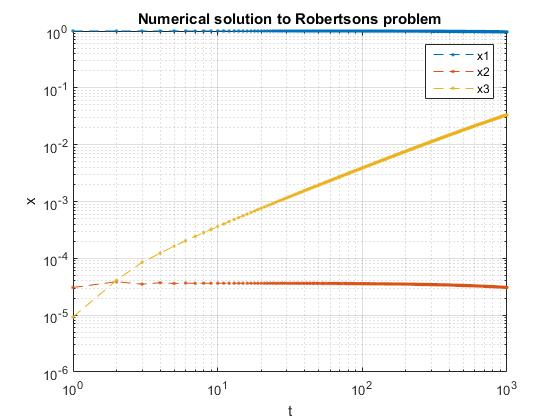
\includegraphics[width=0.7\textwidth,center]{c2121}
\caption{Loglog plot of the solution to the Robertson's Problem.}
\end{figure}

\newpage
\subsection*{2.1.2.2}
In this section, the Robertson's problem shall be solve with two in-build function of Matlab: $ode23$ and $ode23s$.

For the function $ode23$, the equation system is solve on the interval $[0, 1]$ with different relative tolerances and the number of steps taken by $ode23$ is recorded. A loglog plot of the step-sizes against t is plotted and showed below for the smallest relative tolerance. 

For the function $ode23s$, the same process is done on the interval $[0, 1000]$. 

The results are showed below. 

For the function $ode23$. 

\begin{table}
\centering
\begin{tabular}{| c | c | c | c | c |}
\hline 
Relative tolerances & $10^{-3}$ & $10^{-4}$ & $10^{-5}$ & $10^{-6}$ \\
\hline 
Number of steps taken & 867 & 868 & 869 & 869\\
\hline 
\end{tabular}
\end{table}


\begin{figure}[H]
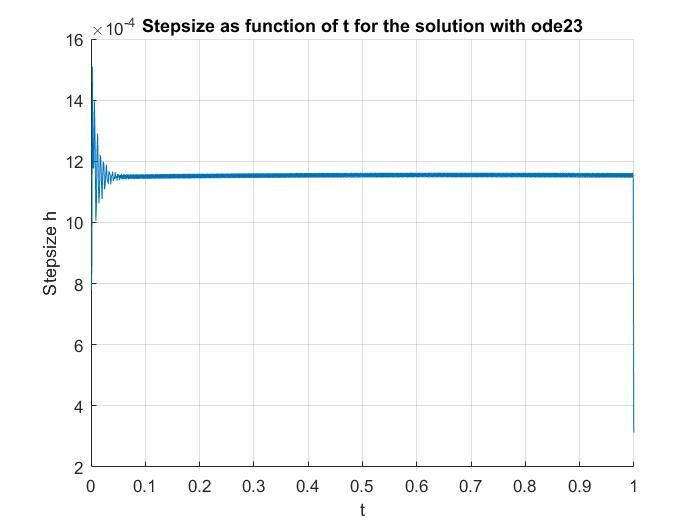
\includegraphics[width=0.7\textwidth,center]{c21221}
\caption{Stepsizes against t for the function ode23}
\end{figure}

For the function $ode23s$. 

\begin{table}
\centering
\begin{tabular}{| c | c | c | c | c |}
\hline 
Relative tolerances & $10^{-3}$ & $10^{-4}$ & $10^{-5}$ & $10^{-6}$ \\
\hline 
Number of steps taken & 31 & 38 & 49 & 62\\
\hline 
\end{tabular}
\end{table}

\begin{figure}[H]
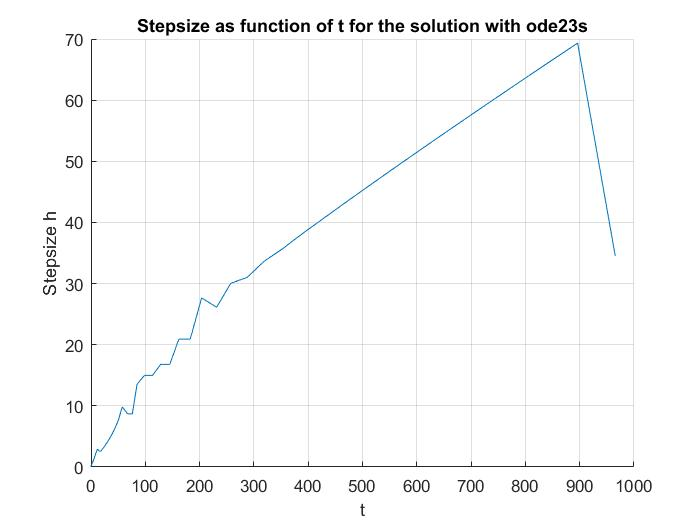
\includegraphics[width=0.7\textwidth,center]{c21222}
\caption{Stepsizes against t for the function ode23s}
\end{figure}

\subsection*{2.1.3.1}
In this problem the particle flow past a cylinder is studied. A long cylinder with radius $R=2$ is placed in an incompressible fluid streaming in the direction of the positive x-axis. The axis of the cylinder is perpendicular to the direction of the flow. The position $(x(t), y(t))$ of a flow particle at time t is determined by the start position $(x(0), y(0))$ and the ODE systems:
\begin{equation}
\frac{dx}{dt} = 1- \frac{R^2(x^2-y^2)}{(x^2+y^2)^2}, \quad \frac{dy}{dt} = -\frac{2xyR^2}{(x^2+y^2)^2}
\end{equation}

The ODE systems are solved with the Runge-Kutta method above with 1000 steps. The result is plotted below. 

\begin{figure}[H]
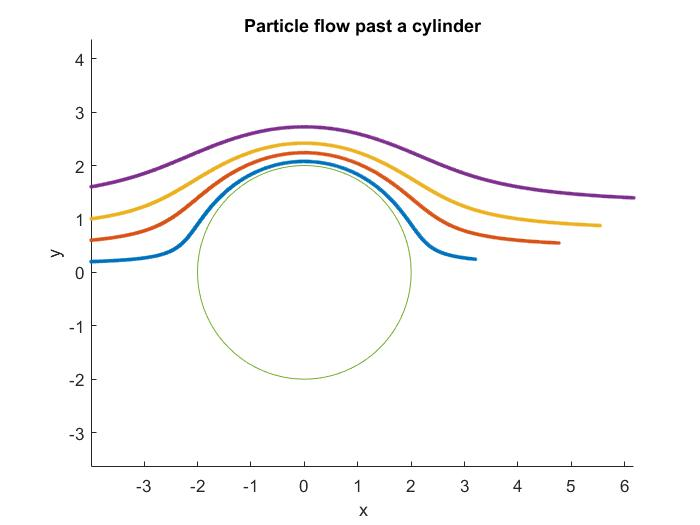
\includegraphics[width=0.7\textwidth,center]{c2131}
\caption{Particle flow around a cylinder.}
\end{figure}


\newpage
\subsection*{2.1.3.2}


Here the differential equations governing the motion of a particle being thrown from the position $(0,1.5)$ with angle $\alpha$ and initial velocity $v_0$ are given. 

The numerical method of choice is Runge-Kutta 3.

Let $u_1=x$, $u_2=\frac{dx}{dt}$, $u_3=y$,$u_4=\frac{dy}{dt}$ then the given ode system can be rewritten on matrix form as 

\begin{equation}
\begin{bmatrix}
\frac{du_2}{dt} \\
\frac{du_4}{dt}
\end{bmatrix} =
\begin{bmatrix}
f_1(u_1,u_2,u_3,u_4) \\
f_2(u_1,u_2,u_3,u_4)
\end{bmatrix}=
\begin{bmatrix}
-ku_2\sqrt[]{u_2^2+u_4^2} \\
-9.81-k|u_4|\sqrt[]{u_2^2+u_4^2}
\end{bmatrix}
\end{equation},


with initial conditions, $u_1(0)=0$, $u_2(0)=20\cos\alpha$,$u_3(0)=1.5$ and $u_4(0)=20\sin\alpha$.

The initial conditions are used to generate a series of values $\{u_i\}_{i=0,1,...,N}$ using the recursion from the RK3 method.

\begin{equation}
\begin{aligned}
\centering
u_i & =u_{i-1}+\frac{h}{6}(K_1+K_2+4K_3),\quad t_k=t_{i-1}+h, \quad i=1,2, ..., N \\
K_1 & =f(t_{i-1},u_{i-1})\\
K_2 & =f(t{_i-1}+h,u_{i-1}+hK_1)\\
K_3 & =f(t_{i-1}+h/2,u_{i-1}+hK_1/4+hK_2/4) 
\end{aligned}
\end{equation}.



Plots of the solution curves for $k=0.02$, $k=0.065$ and $\alpha=[30\quad45\quad 60]$ is shown in figure \ref*{soltraj}.

\begin{figure}
\centering
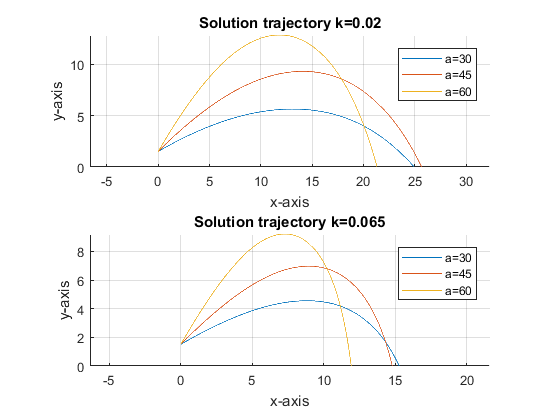
\includegraphics[width=0.6\textwidth]{solution_traj.png}
\caption{Plots of various solution trajectories for a thrown particle.}
\label{soltraj}
\end{figure}














\end{document}



%% Initialization
clear, clc;

%% C.2.1.1
Ns = [10 20 40 80 160 320];
u_end = [];
f = @(u) [0, 1; -1, 1-u(1)^2]*u;
for N = Ns
    h = 1/N;
    u = [1 0]';
    for t = h:h:1
        k1 = f(u);
        k2 = f(u + h*k1);
        k3 = f(u + h*k1/4 + h*k2/4);
        u = u + h/6 * (k1 + k2 + 4*k3);
    end
    u_end = [u_end; u(1)];
end
figure();
loglog(Ns, abs(u_end-u_end(end)));
title('Error against stepsize');
xlabel('Stepsize');
ylabel('Error');
xlim([0 320]);
hold on;
grid on;

%% C.2.1.2.1
Ns = [125 250 500 1000 2000];
u_end = [];
Np = [];
c1 = 0.04;
c2 = 10^4;
c3 = 3*10^7;
f = @(u) [-c1*u(1)+c2*u(2)*u(3); c1*u(1)-c2*u(2)*u(3)-c3*u(2)^2; c3*u(2)^2];
solved = false;
for N = Ns
    h = 1/N;
    u = [1 0 0]';
    sol = zeros(N, 3);
    for t = 1:N
        k1 = f(u);
        k2 = f(u + h*k1);
        k3 = f(u + h*k1/4 + h*k2/4);
        u = u + h/6 * (k1 + k2 + 4*k3);
        sol(t, :) = u;
    end
    if and(not(isnan(u(1))), not(solved))
        solved = true;
        smallest_sol = sol;
        break;
    end
end
figure();
loglog(smallest_sol);
hold on;
grid on;

%% C.2.1.2.2
c1 = 0.04;
c2 = 10^4;
c3 = 3*10^7;
g = @(t, u) [-c1*u(1)+c2*u(2)*u(3);c1*u(1)-c2*u(2)*u(3)-c3*u(2)^2;c3*u(2)^2];
Ns = [];
Nss = [];
Tol = 10.^(-[3, 4, 5, 6]);
for rt = Tol
    [t, y] = ode23(g, [0 1], [1 0 0], odeset('RelTol', rt));
    [ts, ys] = ode23s(g, [0 1000], [1 0 0], odeset('RelTol', rt));
    Ns = [Ns; size(t)*[1 0]'];
    Nss = [Nss; size(ts)*[1 0]'];
end
figure();
hold on;
loglog(t(1:Ns(end)-1), abs(t(2:Ns(end))-t(1:Ns(end)-1)));
grid on;
figure();
hold on;
loglog(ts(1:Nss(end)-1), abs(ts(2:Nss(end))-ts(1:Nss(end)-1)));
grid on;

%% C.2.1.3.1
N = 1000;
R = 2;
f = @(u) [1-R^2*(u(1)^2-u(2)^2)/(u(1)^2+u(2)^2)^2; -2*u(1)*u(2)*R^2/(u(1)^2+u(2)^2)^2]';
nn = 101;
pos = zeros(2, nn);
pos(1, :) = -4;
b = -1.6;
e = 1.6;
pos(2, :) = b:(e-b)/(nn-1):e;
% pos = [-4 0.2; -4 0.6; -4 1.0; -4 1.6];
pos = pos';
figure();
hold on;
axis equal;
for i = 1:size(pos)*[1 0]'
    u = pos(i, :);
    h = 20/N;
    sol = zeros(N, 2);
    for t = 1:N
        k1 = f(u);
        k2 = f(u + h*k1);
        k3 = f(u + h*k1/4 + h*k2/4);
        u = u + h/6 * (k1 + k2 + 4*k3);
        sol(t, :) = u;
    end
    plot(sol(:, 1), sol(:, 2));
end
































%%% C2.1.3.2
clc,clear all,close all
N=1000;
i=1;
for k=[0.02 0.065];
    subplot(2,1,i)
    for a=[30 45 60];
    count=1;
    h = 1/N;
    u = [0 20*cosd(a) 1.5 20*sind(a)]';
    f = @(u) [u(2); -k*u(2)*sqrt((u(2)^2+u(4)^2)); u(4); -9.81-k*abs(u(4))*sqrt((u(2)^2)+(u(4)^2))];

   t=1;
       %while u(3)> -10
    while 1==1
        if u(3) <= 0
            break;
        end
        k1 = f(u);
        k2 = f(u + h*k1);
        k3 = f(u + h*k1/4 + h*k2/4);
        u = u + h/6 * (k1 + k2 + 4*k3);
        sol(t,:)=u;
        t=t+1;
       end
    
    
    axis equal
    hold on
    grid on
    plot(sol(1:t-1,1),sol(1:t-1,3))
    end
    legend('a=30','a=45','a=60')
    grid on
    xlabel('x-axis')
    ylabel('y-axis')
    title(['Solution trajectory k=', num2str(k)])
    i=i+1;
end